\begin{frame}[t]{}
  \vfill\begin{center}{\Huge\color{YaleBlue} The Constrained Mixture Model}
  \end{center}\vfill
\end{frame}

\begin{frame}[t]{One Framework, Many Applications}
  \vfill
  \begin{center}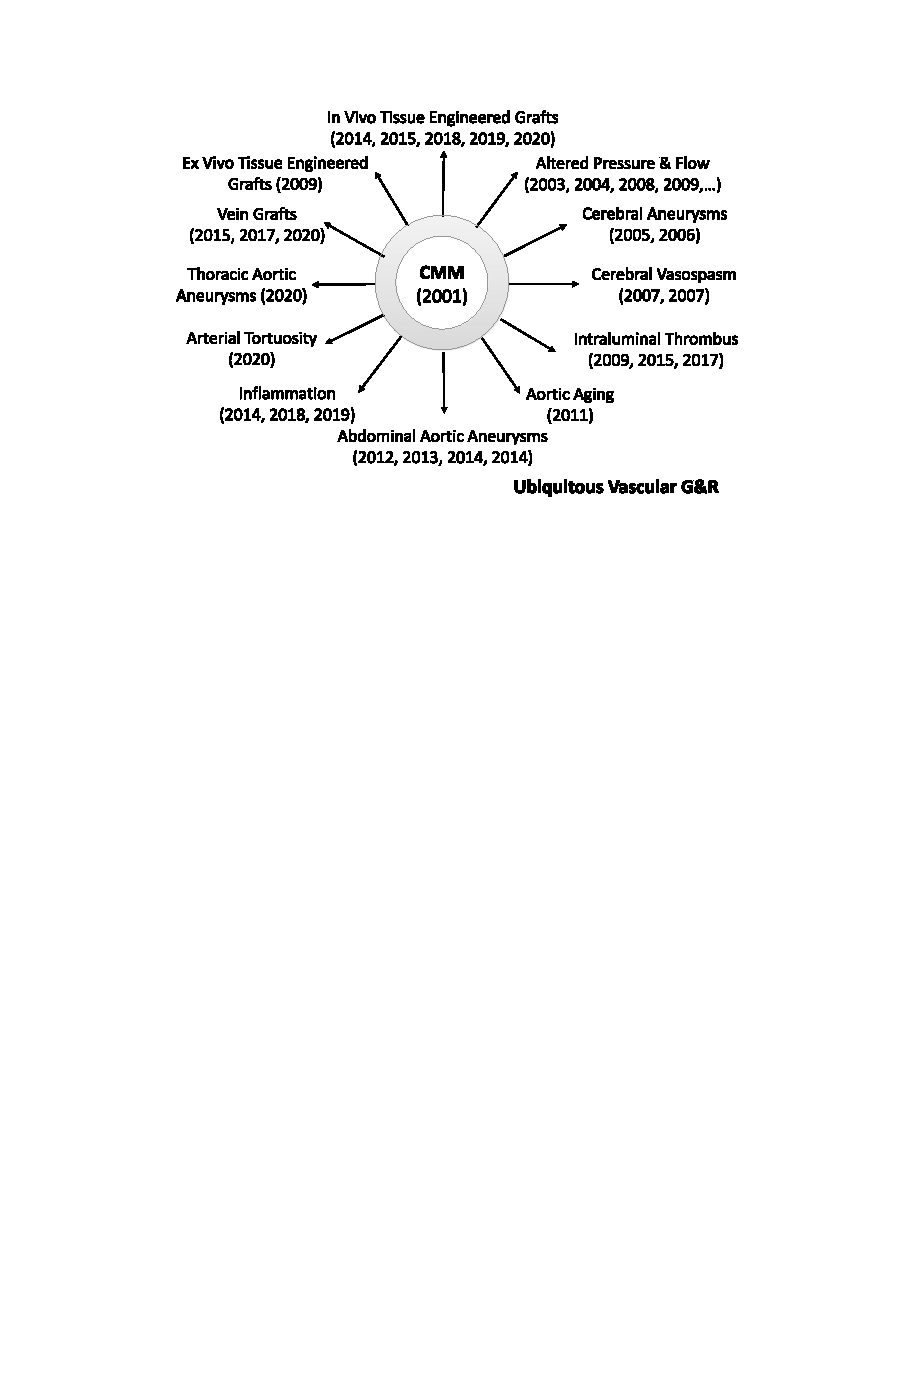
\includegraphics[height=0.9\textheight]{figures/cmm_applications.pdf}\end{center}
  \vfill
  \srccite{Humphrey, J Elasticity (2021)}
\end{frame}

\begin{frame}[t]{The Idea: Track Every Cohort}
  \vfill
  \begin{center}\humphreygr[0.56]\end{center}
  \vspace{-0.1em}
  \begin{center}\footnotesize\color{black!70}
  $\kappa$: configuration \;\textbullet\; $\tau$: deposition time \;\textbullet\;
  $s$: current time \;\textbullet\; $\alpha$: constituent
  \;\textbullet\; $\bm{G}^{\alpha}$: deposition stretch \;\textbullet\;
  $\bm{F}^{\alpha}_{n(\tau)}$: constituent deformation
  \end{center}
  \vfill
  \srccite{Humphrey, J Elasticity (2021)}
\end{frame}

\begin{frame}[t]{Load-Bearing Vessel Constituents}
  \footnotesize
  The wall is a mixture of three constituents, each with a reference \textbf{mass
  fraction} $\phi_0^{\alpha}$ ($\sum_\alpha\phi_0^{\alpha}=1$) and a
  \textbf{deposition stretch} $G^{\alpha}$ --- the prestretch cells lay it down at,
  which \emph{defines} its homeostatic stress
  $\sigma_h^{\alpha}=\sigma^{\alpha}(G^{\alpha})$; the mixture set-point is
  $\bar\sigma_h=\sum_\alpha\phi_0^{\alpha}\sigma_h^{\alpha}$.
  \vspace{0.3em}
  \renewcommand{\arraystretch}{1.3}
  \begin{center}
  \begin{tabular}{@{}p{0.15\textwidth}p{0.28\textwidth}ccp{0.24\textwidth}@{}}
    \toprule
    \textbf{Constituent} & \textbf{Role} & $\phi_0$ & $G^{\alpha}$ & \textbf{law; turnover $1/k_d$}\\
    \midrule
    \textbf{\color{YaleBlue}Elastin} & bears load at low stretch & 0.30 & 1.40 &
      neo-Hooke; \textbf{none} (decades)\\
    \textbf{\color{YaleBlue}Collagen} & stiff, crimped; anti-rupture & 0.35 & 1.08 &
      Fung; fast ($\sim$20\,d)\\
    \textbf{\color{YaleBlue}Smooth muscle} & passive + active; the sensor & 0.35 & 1.20 &
      Fung; fast ($\sim$20\,d)\\
    \bottomrule
  \end{tabular}
  \end{center}
  \vspace{0.3em}
  \textbf{Elastin cannot be renewed} ($k_d^e=0$) --- its loss drives
  \emph{aneurysm}; collagen \& SMC \textbf{turn over}, so the wall can
  \emph{adapt}.
  \srccite{Humphrey, Eberth, Dye, Gleason, J Biomech (2009)}
\end{frame}

\begin{frame}[t]{Every Cohort Shares One Stretch}
  A cohort of $\alpha$ deposited at $\tau$ is laid down at $G^{\alpha}$ and then
  stretches \emph{with the mixture}: every constituent and cohort is
  \textbf{constrained} to the same tissue stretch $\lambda(s)$.
  \dlab{constituent-specific deformation}
  \giveneq{\bm{F}^{\alpha}_{n(\tau)}(s) = \bm{F}(s)\,\bm{F}^{-1}(\tau)\,\bm{G}^{\alpha}(\tau).}
  \zlab{scalar elastic stretch}
  \slboxeq{eq:cohort}{\lambda_{n(\tau)}^{\alpha}(s,\tau) = \frac{\lambda(s)}{\lambda(\tau)} \, G^{\alpha}}
  \srccite{Humphrey, Rajagopal, Math Models Methods Appl Sci (2002)}
\end{frame}

% ---- derivation after Humphrey (2021): mass balance (1) ----------------------
\begin{frame}[t]{Mass Balance}
  Track each constituent's
  \textbf{apparent mass density} $\rho^{\alpha}$ per current
  mixture volume, $\rho=\sum_{\alpha}\rho^{\alpha}$.
  \par\medskip
  Spatial mass balance (one per constituent):
  \giveneq{\frac{\partial\rho^{\alpha}}{\partial s}
     + \underbrace{\operatorname{div}(\rho^{\alpha}\bm{v}^{\alpha})}_{\text{transport}}
     = \underbrace{\bar m^{\alpha}}_{\text{net mass exchange}},
     \qquad \alpha=1,\dots,N.}
  The net rate is \emph{signed}:
  \giveneq{\bar m^{\alpha}=\underbrace{m^{\alpha}}_{\text{production}\ge 0}
     -\underbrace{r^{\alpha}}_{\text{removal}\ge 0}
     \;\begin{cases}
       <0 & \text{atrophy}\\[2pt]
       =0 & \text{maintenance}\\[2pt]
       >0 & \text{growth}
     \end{cases}}
  \srccite{Humphrey, J Elasticity (2021)}
\end{frame}

% ---- assumptions 1 & 2 -> heredity integral (2) ------------------------------
\begin{frame}[t]{From Balance to a Heredity Integral}
  \textbf{Assumption 1 (constrained mixture):} every constituent moves with the
  mixture, $\bm{v}^{\alpha}=\bm{v}$.
  \par\smallskip
  \textbf{Assumption 2 (prescribed rates):} a true production rate
  $m^{\alpha}(\tau)\ge 0$ and a survival fraction $q^{\alpha}(s,\tau)\in[0,1]$.
  Integrating from the distant past to $s$:
  \slboxeq{eq:massher}{\rho^{\alpha}(s)=
     \underbrace{\rho^{\alpha}(0)\,Q^{\alpha}(s)}_{\text{survivors of original material}}
     +\underbrace{\int_{0}^{s} m^{\alpha}(\tau)\,q^{\alpha}(s,\tau)\,\dd\tau}
       _{\text{deposited at }\tau,\ \text{still present at }s}}
  with $Q^{\alpha}(0)=1$. \textbf{Assumption 3:} bulk density is nearly constant,
  $\rho(s)=\rho(0)$ --- mass changes track volume changes.
  \srccite{Humphrey, J Elasticity (2021)}
\end{frame}

\begin{frame}[t]{Linear Momentum Balance}
  A rule-of-mixtures for the stresses (no body forces) satisfies the classical
  linear-momentum balance:
  \giveneq{\operatorname{div}\bm{\sigma}=\rho\,\bm{a}
     \;\;\xrightarrow{\ \text{quasi-static}\ }\;\;
     \operatorname{div}\bm{\sigma}=\bm{0}.}
  \textbf{Quasi-static assumption:} G\&R evolves slowly at every time $s$, so the
  inertia $\rho\bm{a}$ is negligible.
  \srccite{Humphrey, J Elasticity (2021)}
\end{frame}

\begin{frame}[t]{Constitutive Relations: Cauchy Stress}
  In finite elasticity the Cauchy stress follows from a stored-energy function
  $W$ (per unit reference mixture volume):
  \giveneq{\bm{\sigma}(s)=\frac{2}{J}\,\bm{F}(s)\,
     \frac{\partial W(s)}{\partial\bm{C}(s)}\,\bm{F}^{\mathrm{T}}(s),
     \qquad \bm{C}=\bm{F}^{\mathrm{T}}\bm{F},\quad J=\det\bm{F}.}
  Rule of mixtures: $W=\sum_{\alpha}\tilde W^{\alpha}$. Closing the model needs
  \textbf{three constituent-specific relations} --- a \emph{stored energy}
  $W^{\alpha}$, a \emph{production} rate $m^{\alpha}$, and a \emph{removal}
  (survival) $q^{\alpha}$.
  \srccite{Humphrey, J Elasticity (2021)}
\end{frame}

\begin{frame}[t]{Three Constituent-Specific Constitutive Relations}
  \textbf{1.\ Material:} constituent stored energy $W^{\alpha}$: neo-Hookean
  elastin, Fung-type collagen \& smooth muscle (eq.~\eqref{eq:fung}).
  \par\medskip
  \textbf{2.\ Rate of production:} up with wall stress \& inflammation, down
  with wall shear:
  \slboxeq{eq:production}{m^{\alpha}(\tau)=m_o^{\alpha}\big(1
     + K_{\sigma}^{\alpha}\,\Delta\sigma
     - K_{\tau_w}^{\alpha}\,\Delta\tau_w
     + K_{\varphi}^{\alpha}\,\Delta\rho_{\varphi}\big)\ge 0}
  \vspace{-0.4em}
  \begin{center}\footnotesize\color{black!70}
   $\Delta\sigma$: pressure \;\textbullet\; $\Delta\tau_w$: flow \;\textbullet\;
   $\Delta\rho_{\varphi}$: inflammation
  \end{center}
  \textbf{3.\ Rate of removal:} a survival fraction that decays faster under
  stress perturbation:
  \slboxeq{eq:removal}{q^{\alpha}(s,\tau)=\exp\!\Big(\!-\!\int_{\tau}^{s}
     k_o^{\alpha}\big(1+\omega\,\Delta\sigma^{2}(t)+\cdots\big)\,\dd t\Big)\in[0,1]}
  \srccite{Valentin, \ldots, Humphrey, J R Soc Interface (2009)}
\end{frame}

\begin{frame}[t]{Constituent Stored-Energy Functions}
  Each cohort carries its \emph{own} stored energy $W^{\alpha}$, evaluated at its
  elastic deformation
  $\bm{F}^{\alpha}_{n(\tau)}(s)=\bm{F}(s)\,\bm{F}^{-1}(\tau)\,\bm{G}^{\alpha}(\tau)$.
  Summing over cohorts with the \emph{same} heredity structure gives the apparent
  (mixture-level) energy:
  \slboxeq{eq:mixenergy}{\rho\,\tilde W^{\alpha}(s)=
     \underbrace{\rho^{\alpha}(0)\,Q^{\alpha}(s)\,W^{\alpha}\!\big(\bm{F}^{\alpha}_{n(0)}(s)\big)}
       _{\text{original material}}
     +\underbrace{\int_{0}^{s} m^{\alpha}(\tau)\,q^{\alpha}(s,\tau)\,
       W^{\alpha}\!\big(\bm{F}^{\alpha}_{n(\tau)}(s)\big)\,\dd\tau}_{\text{later cohorts}}}
  The mixture energy $W=\sum_{\alpha}\tilde W^{\alpha}$ closes the stress above.
  \srccite{Humphrey, J Elasticity (2021)}
\end{frame}

\begin{frame}[t]{Special Cases: $s=0$ and Homeostasis}
  \textbf{(i) At $s=0$} (just before a perturbation) only original material is
  present, and $Q^{\alpha}(0)=1$:
  \giveneq{\rho\,\tilde W^{\alpha}(0)=\rho^{\alpha}(0)\,W^{\alpha}\!\big(\bm{F}^{\alpha}_{n(0)}(0)\big)
     \;\Rightarrow\;
     \tilde W^{\alpha}(0)=\underbrace{\tfrac{\rho^{\alpha}(0)}{\rho(0)}}_{\phi^{\alpha}(0)}
       W^{\alpha}(0),}
  recovering the rule of mixtures $W(0)=\sum_{\alpha}\phi^{\alpha}(0)\,W^{\alpha}(0)$.
  \par\medskip
  \textbf{(ii) Homeostasis} --- turnover in an \emph{unchanging} configuration, so
  $\bm{F}^{\alpha}_{n(\tau)}(s)=\bm{F}^{\alpha}_{n(0)}(s)$ (independent of $\tau$).
  Then $W^{\alpha}$ factors out and, using the mass balance,
  \slboxeq{eq:homeo}{\rho\,\tilde W^{\alpha}(s)=
     \underbrace{\Big(\rho^{\alpha}(0)Q^{\alpha}(s)+\!\int_{0}^{s}\! m^{\alpha}q^{\alpha}\,\dd\tau\Big)}_{=\;\rho^{\alpha}(s)}
     \,W^{\alpha}\!\big(\bm{F}^{\alpha}_{n(0)}(s)\big)
     \;\Rightarrow\; \tilde W^{\alpha}(s)=\phi^{\alpha}(s)\,W^{\alpha}(s).}
  \srccite{Humphrey, J Elasticity (2021)}
\end{frame}

\begin{frame}[t]{Perfect Maintenance}
  Take \emph{constant} rates: $m^{\alpha}=m_0$, $Q^{\alpha}(s)=e^{-K^{\alpha}s}$,
  $q^{\alpha}(s,\tau)=e^{-K^{\alpha}(s-\tau)}$. The mass balance integrates to
  \giveneq{\rho^{\alpha}(s)=
     \underbrace{\rho^{\alpha}(0)\,e^{-K^{\alpha}s}}_{\text{original decays}}
     +\underbrace{\frac{m_0}{K^{\alpha}}\big(1-e^{-K^{\alpha}s}\big)}_{\text{production accumulates}}.}
  A time-\emph{invariant} density ($\rho^{\alpha}(s)=\rho^{\alpha}(0)$ for all $s$)
  requires the two to balance exactly:
  \slboxeq{eq:perfmaint}{\text{perfect maintenance}\iff
     \frac{m_0}{K^{\alpha}}=\rho^{\alpha}(0).}
  Production $m_0$ then exactly offsets removal $K^{\alpha}\rho^{\alpha}$ ---
  continuous turnover, unchanging tissue.
  \srccite{Valentin \& Humphrey, Phil Trans R Soc A (2009)}
\end{frame}

\begin{frame}[t]{}
  \begin{yourturnbox}{Computational Cost?}
    \qq{At each of $N$ time steps the mixture stress sums over \emph{all} cohorts
    deposited so far. How does the total cost scale with $N$?}
    \qhint{Step $k$ re-sums $\sim k$ stored cohorts; add up $\sum_{k=1}^{N}k$.}
  \end{yourturnbox}
  \vfill
  \begin{center}
  $\displaystyle\sum_{k=1}^{N} k=\frac{N(N+1)}{2}=\mathcal{O}(N^2)$
  \end{center}
  \vfill
\end{frame}


\begin{frame}[t]{}
  \begin{setupbox}{Example --- turnover under hypertension (\texttt{ex03})}
    \sprob{The same artery, now with collagen \& SMC turning over (elastin does
    not). Which constituent grows to carry the load, and does turnover restore the
    set-point? Equilibrium each step:
    $\bar\sigma(\lambda)=\bar\sigma_h\,\gamma\,\lambda^{2}/m$ (load factor $\gamma$,
    mass ratio $m$).}
    \srun{\scodeline{uv run python run.py configs/ex03\_constrained\_mixture.yaml}
      Sets each constituent's \texttt{turnover\_days} ($1/k_d$), \texttt{gain}
      ($K_\sigma$), and the \texttt{insult} --- hypertension ($\gamma$) or aneurysm
      (\texttt{elastin\_surviving}).}
    \sstudy{\scodeline{... --set model.constituents.collagen.gain=3.0}}
  \end{setupbox}
\end{frame}

% ---- interactive coding exercise: ex03 -------------------------------------
\begin{frame}[t]{}
  \begin{yourturnbox}{Constrained mixture}
    \qq{Does the same tissue \emph{adapt} to hypertension but \emph{run away} on
    the aneurysm insult? Which constituent grows to carry the load elastin used
    to bear?}
    \qhint{Try turnover 10 / 20 / 70 d and gain 0.3 / 1.0 / 3.0. Faster turnover
    and higher gain reach the new state sooner; watch which insult the tissue can
    absorb.}
  \end{yourturnbox}
\end{frame}

\begin{frame}[t]{}
  \begin{answerbox}{Constrained mixture}
    Mild hypertension \textbf{adapts}: collagen and SMC grow, tissue stress returns
    to homeostatic. A severe elastin insult can \textbf{run away}. Faster turnover
    / higher gain reach the new state sooner.
  \end{answerbox}
  \vspace{-0.2em}
  \bigfigw{fig03_constrained_mixture.pdf}{0.98\linewidth}{Your run: under
  hypertension collagen/muscle grow, elastin dilutes, stress returns to set-point.}
\end{frame}
